\large
Durante lo svolgimento di un caso di studio, verrà replicato il grafo clusterizzato della \figurename{\ref{fig:springExample}} utilizzato nel capitolo 6 a titolo di esempio per delucidare il lettore sulle forze in gioco tra nodi e cluster nel metodo spring-embedding supponendo il cluster che contiene tutto il resto del grafo definito come radice dell'albero di inclusione $T$

\section{Creazione e modifica}
\begin{figure}[!htb]
	\begin{center}
		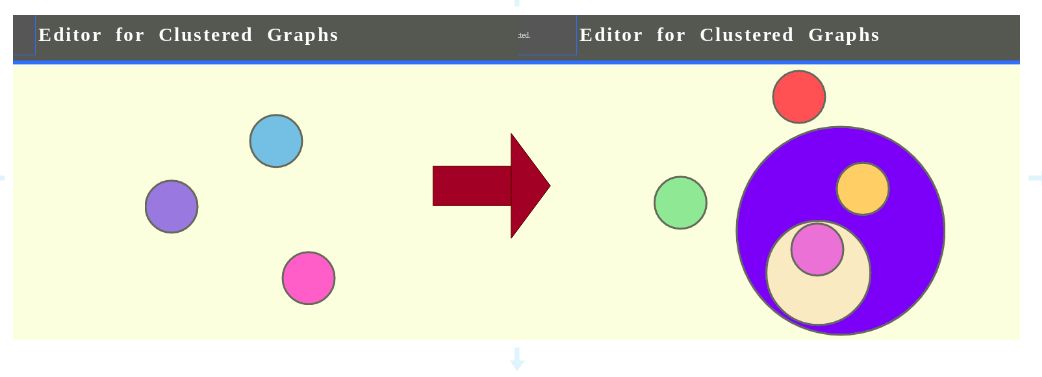
\includegraphics[width=1 \linewidth]{figure/prePostEdit}
	\end{center}
	\caption{cluster prima e dopo l'inserimento di sotto-cluster \label{fig:prePostEdit}}
\end{figure}
Dopo il log-in iniziale in cui viene direttamente creato il cluster radice, essendo rappresentato dal piano di lavoro \#cgraph stesso. Essendo un caso di studio del quale non si possiede un file json prestabilito ed è differente da ogni modello incluso nell'editor risulta necessaria la creazione partendo da una pagina bianca. Detto ciò anche l'oggetto \textit{clusteredGraph} sarà completamente vuoto e l'utente inizierà ad utilizzare il sistema partendo dalla creazione dei cluster di livello uno. Definiti questi oggetti si passerà alle interazioni per la creazioni dei cluster figli. In questo caso sarà necessaria dunque una interazione per ogni cluster figlio che si vorrà definire poiché ogni volta il sistema dovrà aggiornare la visualizzazione dei dati creati in quanto cambieranno il raggio $r_c$ $\forall$cluster trasformato e nuove forze dovranno essere inserite. La creazione dei figli di un cluster può essere vista nella \figurename{\ref{fig:prePostEdit}} in cui si mette a confronto la visualizzazione dei dati precedente e postuma all'inserimento dei sotto-cluster. 
Come si nota prima e dopo le operazioni di inserimento sono state cambiate automaticamente dalla funzione di redraw le posizioni degli oggetti e manualmente, mediante una interazione da parte dell'utente, i colori degli oggetti mediante l'operazione vista nel capitolo.
\begin{figure}[!htb]
	\begin{center}
		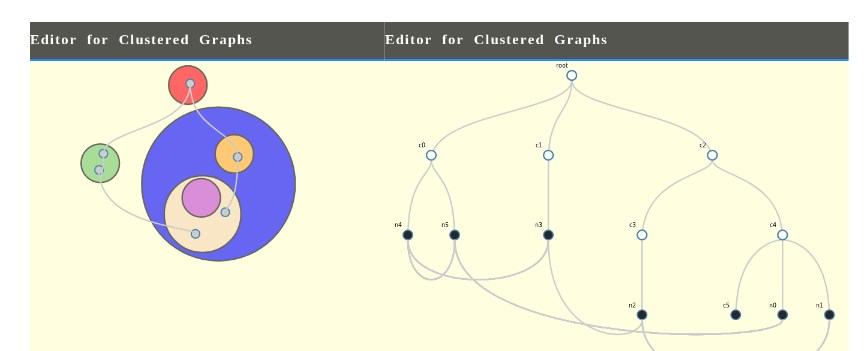
\includegraphics[width=1 \linewidth]{figure/views}
	\end{center}
	\caption{visualizzazione del grafo rappresentato nelle due visualizzazioni \label{fig:views}}
\end{figure}
Si passa ora all'introduzione di nodi e delle loro connessioni. Concludendo poi con qualche operazione di modifica e spostamento sono mostrate nella  \figurename{\ref{fig:views}} il compimento del grafo richiesto e della sua visualizzazione in entrambi gli encode disponibili. 
Si nota inoltre che vi è un cluster senza nodi e non connesso a nulla. L'utente può decidere inoltre di eliminarlo oppure lasciarlo nel caso di future modifiche e decidere di inserire un testo descrittivo per quel particolare oggetto. Entrambe le operazioni sopra citate possono essere eseguite come mostrato nella figura \figurename{\ref{fig:deleteOrAddText}} in cui sono state eseguite l'operazione di rimozione dell'oggetto superfluo a sinistra oppure l'operazione di descrizione a destra.

\begin{figure}[!htb]
	\begin{center}
		\vspace{1cm}
		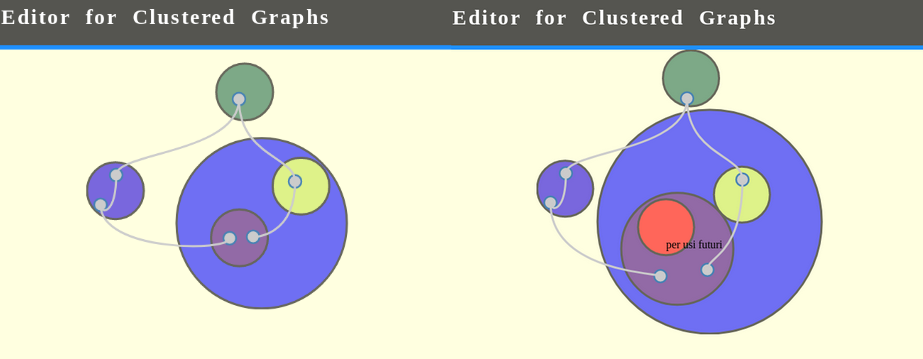
\includegraphics[width=1 \linewidth]{figure/deleteOrAddText}
	\end{center}
	\caption{rimozione o aggiunta di un testo su un cluster\label{fig:deleteOrAddText}}
\end{figure}
Creato il grafo clusterizzato richiesto l'utente può salvare il suo lavoro in un file json che ne descrive la struttura. Il file creato al salvataggio sarà lo stesso che in \figurename{\ref{fig:saveJson}}. In questo modo nelle volte future in cui si dovranno eseguire modifiche o ulteriori creazioni di oggetti non sarà necessario ricreare completamente la struttura ma basterà caricare i progressi salvati nella sessione precedente risparmiando tempo ed imperfezioni. È inoltre possibile come già visto un salvataggio del grafo clusterizzato in un file con estensione .png. La resa della visualizzazione resta comunque il compito principale dell'utente ed è variabile al tempo impiegato per la creazione degli oggetti e per il loro posizionamento esatto. Per questo se si hanno esigenze specifiche riguardanti punti esatti e colorazioni predefinite si consiglia sempre di cominciare una sessione di lavoro su un piano vuoto.
\begin{figure}[!htb]
	\begin{center}
		\vspace{1cm}
		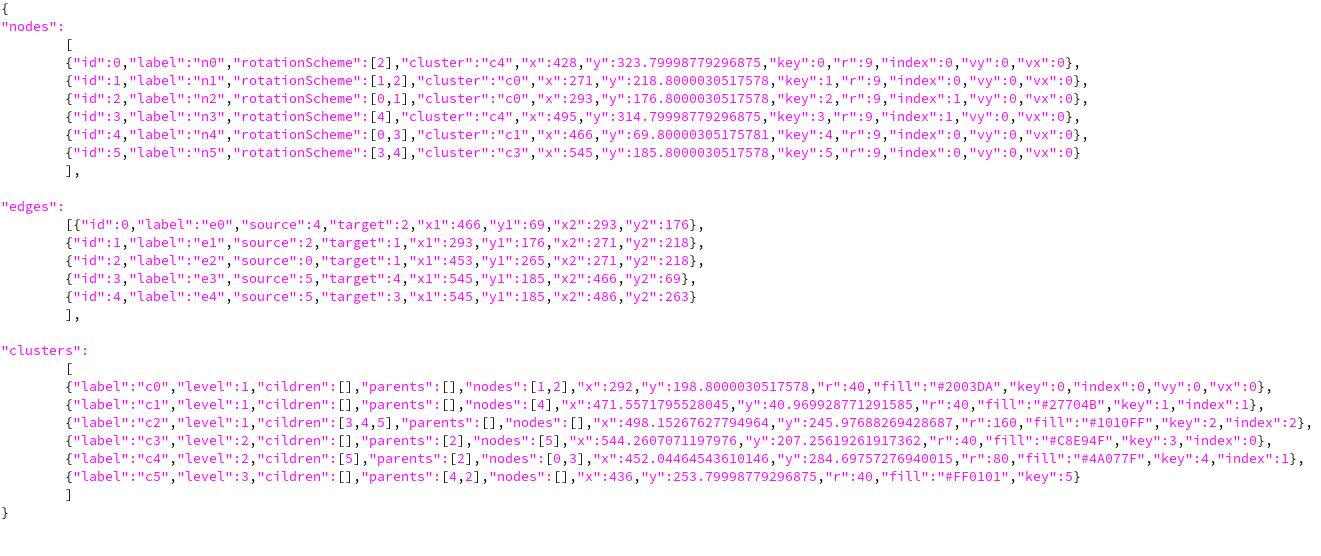
\includegraphics[width=1.1 \linewidth]{figure/saveJson}
	\end{center}
	\caption{Json riferito al salvataggio della struttura del caso di studio\label{fig:saveJson}}
\end{figure}
\newpage
\section{Riduzione e ripresa del grafo}
Terminate le operazioni di creazione degli oggetti e modifiche varie, l'utente decide di rendere il grafo della \figurename{\ref{fig:views}} flat. Supponendo che l'utente abbia scelto di eliminare il cluster senza nodi, mediante una ulteriore interazione è possibile eseguire l'operazione vista nel capitolo precedente. Il risultato è quello mostrato nella figura \figurename{\ref{fig:treeAfterFlat}} mediante la quale si vede il risultato dell'istanza equivalente al grafo clusterizzato.
\begin{figure}[!htb]
	\begin{center}
		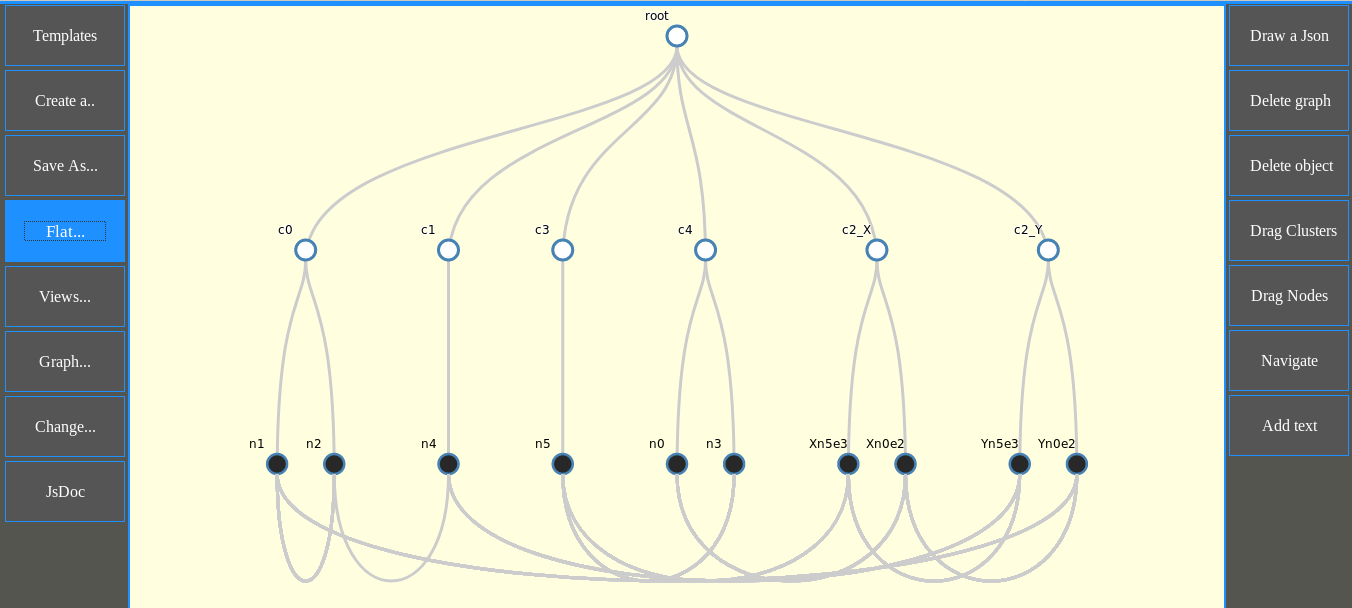
\includegraphics[width=0.8 \linewidth]{figure/treeAfterFlat}
	\end{center}
	\caption{Visione nella treeView dell'istanza flat del grafo clusterizzato\label{fig:treeAfterFlat}}
\end{figure}
Da ora è possibile procedere in due strade:
\begin{itemize}
	\item Analizzare l'istanza e salvare la struttura dati ricevuta sempre mediante file json come risultato ottenuto dalla sessione di lavoro;
	\item Ritornare allo stato della sessione precedente quella di flattizzazione.
\end{itemize}

È infatti possibile per l'utente continuare la modifica del grafo e ritornare ad avere i dati e la conseguente visualizzazione precedenti l'operazione di riduzione nell'istanza equivalente. Analizzando la graphView dopo la flattizzazione il risultato sarà non dissimile da quello riportato nella \figurename{\ref{fig:graphAfterFlat}}. In questo caso sono state ulteriormente applicate delle etichette per consentire con maggior rapidità di conoscere i cluster aggiunti durante il processo di flattizzazione e sono state eseguite operazioni di spostamento per una migliore rappresentazione.

\begin{figure}[!htb]
	\begin{center}
		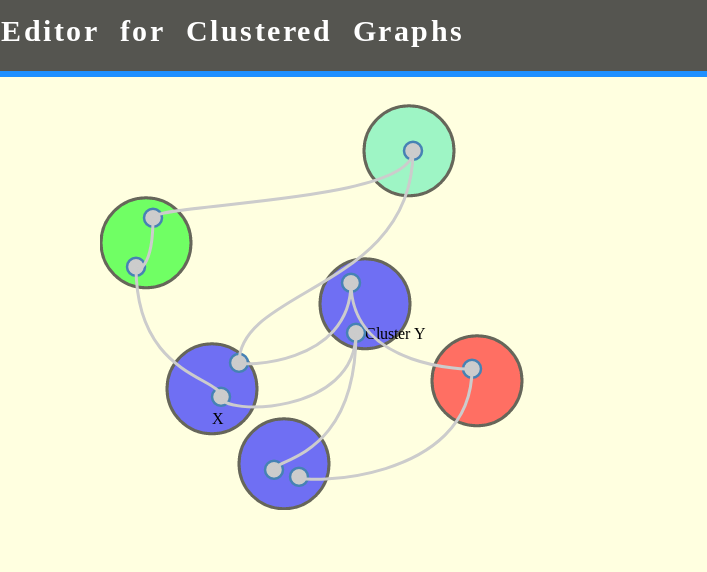
\includegraphics[width=0.8 \linewidth]{figure/graphAfterFlat}
	\end{center}
	\caption{Visione nella graphView dell'istanza flat del grafo clusterizzato\label{fig:graphAfterFlat}}
\end{figure} 